\clearpage
\section{方向光照不亮兔子}

打开 Stanford Bunny，保留主相机、兔子和地面，删掉点光源，让这盏方向光独自照亮场景。旧版的 Lit 面板全黑。按同一机位截取第 24 帧，底色图已经画出了兔子，光照图里最大的 RGB 分量却为零。把剩下的方向光也删掉，离线烘焙出来的文件竟然一字节都没变。绘制与烘焙都遗漏了同一盏灯，单独调整曝光很难找到原因。

\begin{figure}[H]\centering
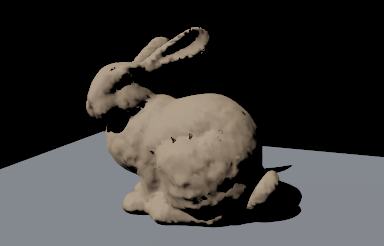
\includegraphics[width=.58\linewidth]{../../../output/validation/directional-light/bunny-after.png}
\caption{修复后同一机位的场景面板。扫描 $384\times246$ 个像素，其中 42,964 个像素至少有一个线性 RGB 分量超过 0.01。这里用 0.01 计数，便于把很暗的边缘与明显受光的区域分开。}
\end{figure}

\noindent{\small C++，\path{RedflagForge/src/LightingPreview.cpp} 的 \texttt{CollectLights}。旧版只遍历下面这一类实体。}
\begin{Code}
// PointLightComponent 只会选出点光源，场景里的方向光没有进入数组。
scene.GetRegistry().view<TransformComponent, PointLightComponent>()
\end{Code}

修复分了两处。编辑器把方向光一起交给显卡；着色器再按灯的类型解释这份数据。对点光源，要从着色点指向灯的位置。对方向光，直接使用已算好的单位方向即可。把新接口造出的方向光交给旧着色器，两面材质相同、正对太阳的墙竟会因远近而得到 0.02464 和 0.00334 两个读数。改好着色器后，两处红色都为 0.49529。打开阴影后，挡板覆盖的半边读作零。回放中事件 8 算逐灯结果，事件 33 算分簇结果，两个输出吻合。\href{run:../validation/directional/DirectionalLight_capture.rdc}{墙面试验的 RenderDoc 帧}

另一次排查从文件开始。将灯牌模型引用的图片暂时移走，旧版继续按材质颜色计算，随后覆盖了原有烘焙。现在点击烘焙时，编辑器重新读取模型及其贴图。如果读不到其中一张图，会给出文件名。补回图片再试，得到的文件与最初烘焙的内容相同；命令行遇到同样的错误则返回失败。\href{run:../validation/directional-light/probe-textures.json}{缺图、损坏与恢复的实测记录}

保持镜头不动，再给墙换一张法线贴图，是另一个容易漏掉的操作。贴图改变了像素受光的方向，旧面板却继续显示上一张颜色图。现在编辑器记录实际送入显卡的法线图，换图或给原贴图写入新像素都会触发重画。探针按三角形的法线计算，所以这项编辑可以保留之前的烘焙。\href{run:../profiling/probe-materials/editor-edits.tsv}{固定镜头下的改材质测试}
